\section{Sample surface microscopy}
\label{sec:microscopy}

Take a picture of the non-radiative defects
of the sample
under the microscope.
For this connect the pump light
with the microscope illumination,
and place the camera,
including a long-pass filter
so we see only the photoluminescence
and block the pump,
as illustrated in Fig.~\ref{img:microscopy}.

Note:
Whenever you change the fiber
connected to the pump diode,
ensure the fiber is intact --
to avoid damages portrayed in Fig.~\ref{img:burnt} --
and make sure
to have the best possible
diode-to-fiber coupling.
For the first task
use the fiber inspection microscope.
For the latter
(see diode manual!)
apply a certain pump,
unscrew the fiber connection
at the pump diode module,
and turn the fiber end
while observing the change in output power.
Lock it for the maximum configuration.

With a microscope magnification of $5\times$,
take a picture of all four corners.
For this you can use
the fully equiped NI-MAX,
which came along with the other NI drivers,
see Fig.~\ref{img:ni_max}.
The overlapping parts of these images
allow you to staple together
the whole photograph.

\begin{figure}
\centering
\subfigure{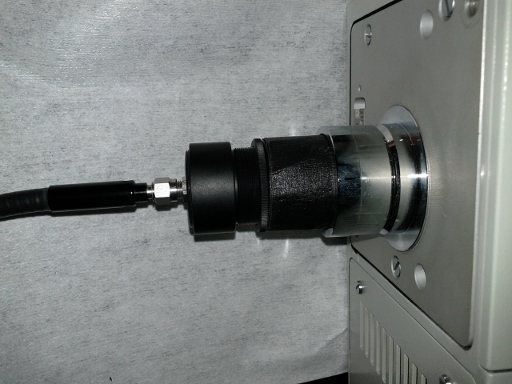
\includegraphics[width=6cm]{img/micro_illum.jpg}}
\subfigure{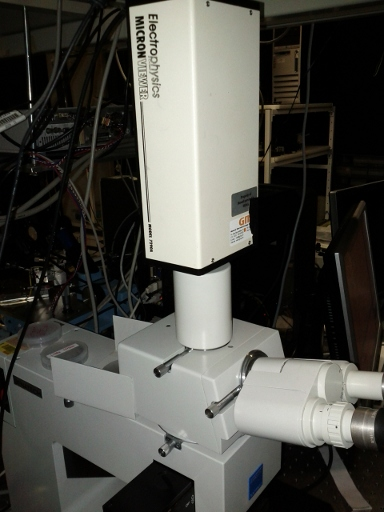
\includegraphics[width=6cm]{img/micro_cam.jpg}}
\caption{Direct the pump light to the microscope for illumination.
With this light source,
and a long-pass filter on the camera,
the non-radiative defects are directly visible.}
\label{img:microscopy}
\end{figure}

\begin{figure}
\centering
\subfigure{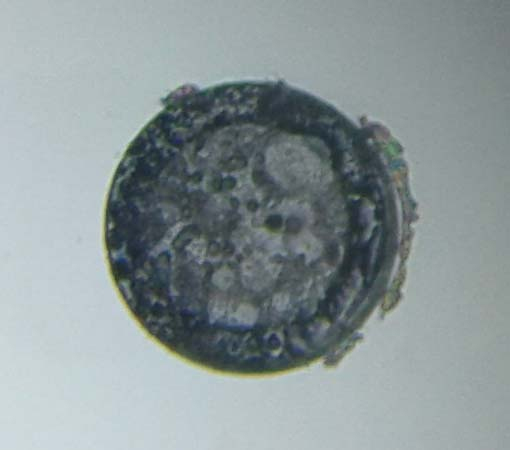
\includegraphics[width=6cm]{img/fiber_bad.jpg}}
\subfigure{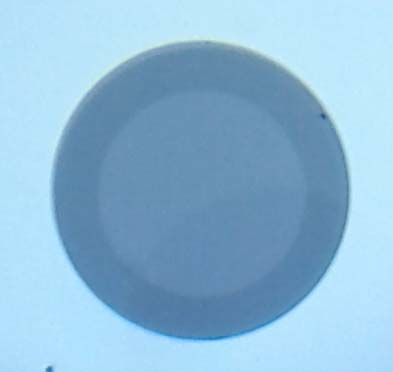
\includegraphics[width=6cm]{img/fiber_good.jpg}}
\caption{Left: This fiber end is burnt; it delivers a beam of bad quality.
Rigth: This is how all fiber interfaces are supposed like; it is intact.}
\label{img:burnt}
\end{figure}

\begin{figure}
\centering
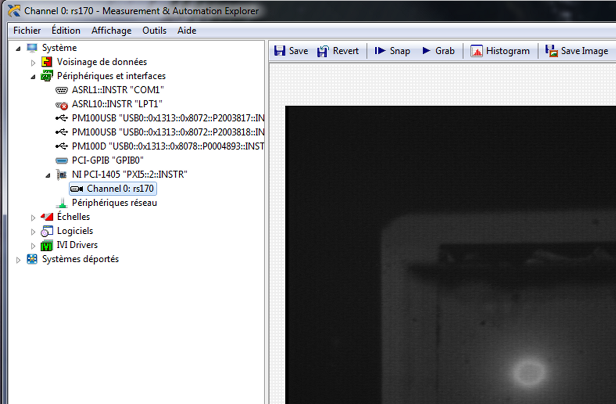
\includegraphics[width=10cm]{img/ni-max.png}
\caption{National Instrument's measurement and automation explorer
(NI MAX) allows us to control the camera.
With ``Grab'' you activate the real-time image feed.
Once the sample is placed as wished, click ``Grab'' again
to stop the broadcast,
and save the image.
To find this software, open the start menu and type ``ni max''.}
\label{img:ni_max}
\end{figure}



